\documentclass[12pt]{article}
\usepackage{preamble}

\pagestyle{fancy}
\fancyhead[LO,LE]{Теория вероятности}
\fancyhead[CO,CE]{26.11.2024}
\fancyhead[RO,RE]{Лекции Блаженова А. В.}

\fancyfoot[L]{\scriptsize исходники найдутся тут: \\ \url{https://github.com/pelmesh619/itmo_conspects} \Cat}

\begin{document}
    \section{Лекция 13}

    \subsection{Математическое ожидание и дисперсия случайного вектора}
    
    $\letsymbol \vec{\xi} = (\xi_1, \dots, \xi_n)$ - случайный вектор, 
    $\forall 1 \leq i \leq n \ \xi_i$ - случайная величина

    \Def Математическим ожиданием случайного вектора называется вектор с координатами 
    из математических ожиданий его компонент: $E\vec{\xi} = (E\xi_1, \dots, E\xi_n)$

    \Def Дисперсией (или матрицей ковариаций) случайного вектора называется матрица
    $D\vec{\xi} = E(\vec{\xi} - E\vec{\xi})^T \cdot (\vec{\xi} - E\vec{\xi})$, состоящая
    из элементов $d_{i, j} = \cov (\xi_i, \xi_j)$. В частности $d_{i, i} = \cov (\xi_i, \xi_i) = D\xi_i$

    \subsection{Функции от двух случайных величин}

    \begin{MyTheorem}
        \Ths Пусть $\xi_1, \xi_2$ - случайные величины с общем плотностью $f_{\xi_1, \xi_2}(x, y)$, и есть функция
        $g(x, y) \ : \ \Real^2 \rightarrow \Real$. Тогда случайная величина $\eta = g(\xi_1, \xi_2)$ имеет
        функцию распределения $F_{\eta}(z) = \iint_{D_z} f(x, y)dxdy$, 
        где $D_z = \{(x, y) \in \Real^2 \ | \ g(x, y) < z\}$
    \end{MyTheorem}

    \begin{MyProof}
        $F_\eta = p(\eta < z) = p(g(\xi_1, \xi_2) < z) = p((\xi_1, \xi_2) \in D_z) = \iint_{D_z} f(x, y) dxdy$
    \end{MyProof}

    \begin{minipage}{\textwidth}
        \begin{wrapfigure}{r}{0pt}
            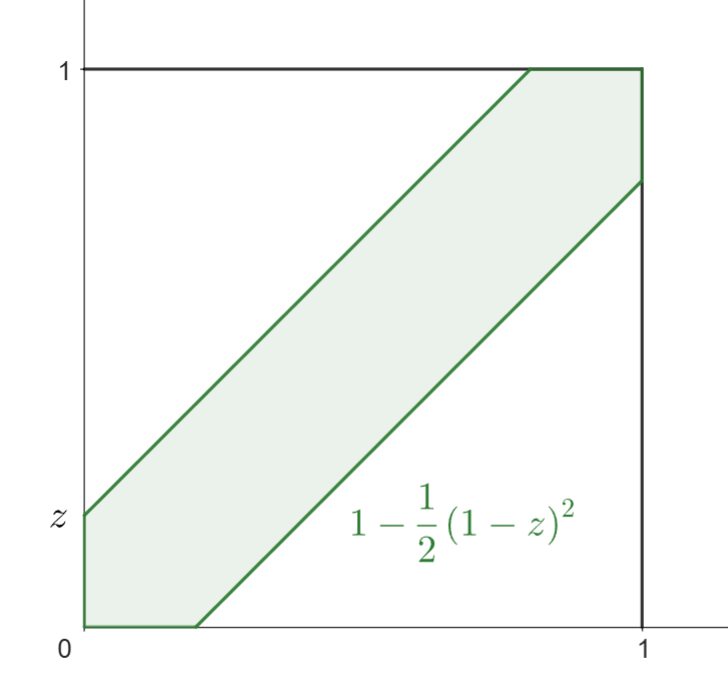
\includegraphics[width=5cm]{probtheory/images/probtheory_2024_11_26_1}
        \end{wrapfigure}

        \ExN{Задача о встрече} двое договорились встретится между 12:00 и 13:00. Случайная величина $\eta$ - 
        время ожидания. Найти функцию распределения

        $\xi_1$ - время прихода первого, $\xi_2$ - второго; $\xi_1, \xi_2 \in U(0, 1)$, они независимы, 
        $\forall x, y \in [0, 1] \ f_{\xi_1}(x) = 1, f_{\xi_2}(y) = 1$

        Поэтому $f_{\xi_1, \xi_2}(x, y) = f_{\xi_1}(x) f_{\xi_2}(y) = 1, (x, y) \in [0, 1] \times [0, 1]$

        $\eta = |\xi_1 - \xi_2| \Longrightarrow D_z = \{(x, y) \in \Real^2 \ | \ |x - y| < z\}$

        $F_\eta = \iint_{D_z} f_{\xi_1, \xi_2}(x, y) dxdy = \iint_{D_z} dxdy = 1 - 2 \cdot \frac{1}{2} (1 - z)^2 = 
        2z - z^2, \ z \in [0, 1]$
    \end{minipage}

    \begin{MyTheorem}
        \Ths $\letsymbol \xi_1, \xi_2$ - независимые абсолютно непрерывные случайные величины с плотностями
        $f_{\xi_1}(x)$ и $f_{\xi_2}(y)$

        Тогда плотность суммы $\xi_1 + \xi_2$ равна $f_{\xi_1 + \xi_2}(t) \int_{-\infty}^\infty 
        \underset{\text{т. н. свертка}}{\underbrace{f_{\xi_1}(x) f_{\xi_2}(t - x)}} dx$
    \end{MyTheorem}

    \begin{MyProof}
        \begin{minipage}{\textwidth}
            \begin{wrapfigure}{r}{0pt}
                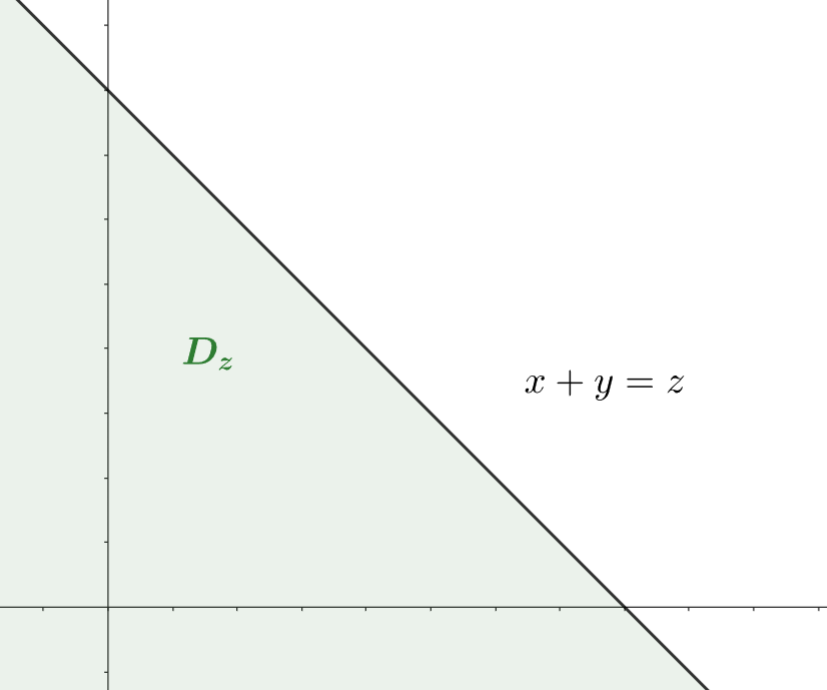
\includegraphics[width=5cm]{probtheory/images/probtheory_2024_11_26_2}
            \end{wrapfigure}
            
            Так как случайные величины $\xi_1$ и $\xi_2$ независимы, то $f_{\xi_1, \xi_2}(x, y) = f_{\xi_1}(x) f_{\xi_2}(y)$

            И согласно предыдущей теореме $F_{\xi_1 + \xi_2}(z) = \iint_{D_z} f_{\xi_1, \xi_2}(x, y) dxdy = 
            \iint_{D_z} f_{\xi_1}(x)f_{\xi_2}(y) dxdy$, где $D_z = \{(x, y) \in \Real^2 \ | \ x + y < z\}$

            $F_{\xi_1 + \xi_2}(z) = \int_{-\infty}^\infty dx \int_{-\infty}^{z - x} f_{\xi_1}(x)f_{\xi_2}(y) dy = \\
            \left[\begin{matrix}y = t - x; & dy = dt; & t = y + x \\ t(-\infty) = -\infty; & t(z - x) = z & \end{matrix}\right] = \\
            \int_{-\infty}^{\infty} f_{\xi_1}(x) dx \int_{-\infty}^z f_{\xi_2}(t - x) dt = \\
            \int_{-\infty}^z \left(\int_{-\infty}^\infty f_{\xi_1}(x)f_{\xi_2}(t - x) dx\right) dt \Longrightarrow
            f_{\xi_1 + \xi_2}(t) = \int_{-\infty}^\infty f_{\xi_1}(x)f_{\xi_2}(t - x) dx$
        \end{minipage}
    \end{MyProof}

    Следствие: сумма двух независимых абсолютно непрерывных случайных величин также имеет абсолютно 
    непрерывное распределение

    \Notas Условие независимости существенно, контр-пример: $\xi_1; \xi_2 = -\xi_1$, тогда $\xi_1 + \xi_2 \equiv 0$

    \subsection{Сумма стандартных распределений. Устойчивость относительно суммирования}

    \Def Если сумма двух независимых случайных величин одного типа распределения также будет этого же типа,
    то говорят, что распределение устойчиво относительно суммирования

    \ExN{1} $\xi \in B_{n, p}; \eta \in B_{m, p}$. Тогда ясно, что $\xi + \eta \in B_{n + m, p}$ 
    (по определению биномиального распределения $B_{n, p}$ - число успехов из $n$ испытаний, где $p$ - вероятность успеха)

    \ExN{2} $\xi \in \Pi_{\lambda}, \eta \in \Pi_{\mu}$, они независимы. Тогда $\xi + \eta \in \Pi_{\lambda + \mu}$

    \begin{MyProof}
        $\xi + \eta = 0, 1, 2, 3, \dots \quad \letsymbol k \geq 0$. 
        Тогда $p(\xi + \eta = k) = \sum^k_{i = 0} P(\xi = i, \eta = k - i) = 
        \sum^k_{i = 0} P(\xi = i) P(\eta = k - i) = \sum_{i = 0}^k \frac{\lambda^i}{i!} e^{-\lambda} \frac{\mu^{k - i}}{(k - i)!} e^{-\mu} = 
        e^{-\lambda - \mu} \sum_{i = 0}^k \frac{\lambda^i \mu^{k - i}}{i! (k - i)!} = 
        e^{-\lambda - \mu} \frac{1}{k!} \sum_{i = 0}^k \frac{\lambda^i \mu^{k - i} k!}{i! (k - i)!} = 
        e^{-\lambda - \mu} \frac{1}{k!} \sum_{i = 0}^k \lambda^i \mu^{k - i}C_k^i = 
        e^{-\lambda - \mu} \frac{(\lambda + \mu)^k}{k!} \Longrightarrow \xi + \eta \in \Pi_{\lambda + \mu}$
    \end{MyProof}

    \ExN{3} $\xi, \eta \in N(0, 1)$ и независимы. Тогда $\xi + \eta \in N(0, 2)$

    \begin{MyProof}
        $f_{\xi}(x) = \frac{1}{\sqrt{2\pi}} e^{-\frac{x^2}{2}}; f_\eta(y) = \frac{1}{\sqrt{2\pi}} e^{-\frac{y^2}{2}}$

        По формуле свертки $f_{\xi + \eta}(t) = \int_{-\infty}^{\infty} \frac{1}{\sqrt{2\pi}} e^{-\frac{x^2}{2}} \frac{1}{\sqrt{2\pi}} e^{-\frac{(t - x)^2}{2}} = 
        \frac{1}{2\pi} \int e^{-(x^2 - tx + \frac{t^2}{2})} = \frac{1}{2\pi} e^{-\frac{t^2}{4}} \int_{-\infty}^\infty e^{-(x^2 - tx + \frac{t^2}{4})} dx = 
        \frac{1}{2\pi} e^{-\frac{t^2}{4}} \int_{-\infty}^\infty e^{-(x - \frac{t}{2})^2} d(x - \frac{t}{2}) = 
        \frac{1}{2\pi} e^{-\frac{t^2}{4}} \sqrt{\pi} = \frac{1}{\sqrt{2}\sqrt{2\pi}} e^{-\frac{t^2}{2(\sqrt{2})^2}} 
        \Longrightarrow \xi + \eta \in N(0, 2)$
    \end{MyProof}

    \ExN{4} В общности для независимых $\xi \in N(a_1, \sigma^2_1), \eta \in N(a_2, \sigma_2^2) \ \xi + \eta \in N(a_1 + a_2, \sigma_1^2 + \sigma_2^2)$ 

    \ExN{5} Равномерное распределение неустойчиво относительно суммирования, контрпример:

    $\xi, \eta \in U(0, 1)$ - независимы

    $\forall x, y \in [0, 1] \ f_{\xi}(x) = 1, f_\eta(y) = 1$ и $f_{\xi, \eta}(x, y) = 1$

    По первой теореме $F_{\xi, \eta}(x, y) = \iint_{D_z} f_{\xi, \eta}(x, y) dxdy = \iint_{D_z} dxdy = S_{D_z}$, где $D_z = \{(x, y) \ | \ x + y < z\}$

    \smallvspace

    \begin{multicols}{2}
        \begin{center}
            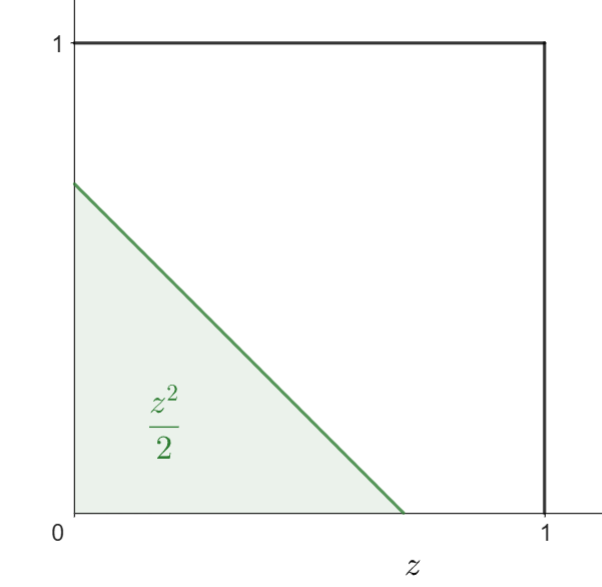
\includegraphics[height=6cm]{probtheory/images/probtheory_2024_11_26_3}

            а) $0 < z \leq 1$
        \end{center}

        \begin{center}
            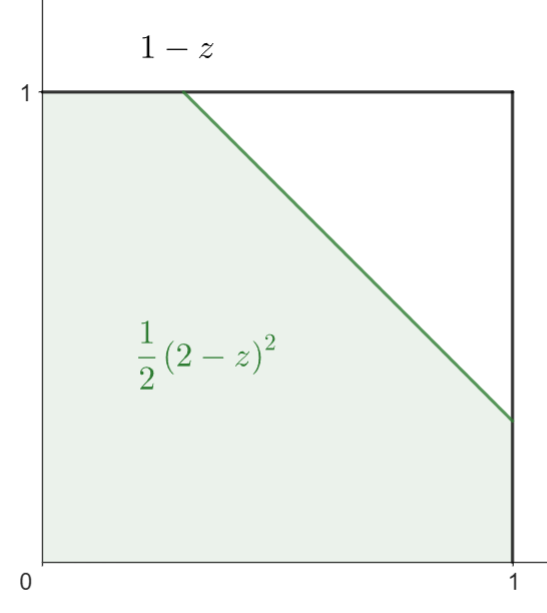
\includegraphics[height=6cm]{probtheory/images/probtheory_2024_11_26_4}

            б) $1 < z \leq 2$
        \end{center}
    \end{multicols}

    \smallvspace

    $S_{D_z} = \begin{cases}0, & z < 0 \\ \frac{z^2}{2}, & 0 \leq z \leq 2 \\ 1 - \frac{1}{2}(2 - z)^2 & 1 \leq z \leq 2 \\ 0, & z > 2\end{cases}$

    $f_{\xi + \eta}(z) = \begin{cases}0, & z < 0 \\ z, & 0 \leq z \leq 2 \\ 2 - z & 1 \leq z \leq 2 \\ 0, & z > 2\end{cases} \not\equiv C \Longrightarrow \xi + \eta$ не имеют равномерное распределение

    \Nota FUN FACT: сумма нескольких величин с равномерным распределением приближается к нормальному распределению

    \subsection{Условное распределение}

    \Def Условным распределением случайной величины из системы случайных величин $(\xi, \eta)$ 
    называется ее распределение, найденное при условии, что другая случайная величина приняла 
    определенное значение. Обозначается $\xi | \eta = y$

    \DefN{A}: Условным математическим ожиданием (обозначается $E(\xi | \eta = y)$) называется 
    математическим ожиданием случайной величины $\xi$ при соответствующем условном распределении

    \subsubsection{I. Условное распределение в дискретной системе двух случайных величин}

    Пусть $(\xi, \eta)$ задана законом распределения:

    \begin{tabular}{c|c|c|c|c}
        $\xi \backslash \eta$ & $y_1$ & $y_2$ & $\dots$ & $y_m$ \\
        \hline
        $x_1$ & $p_{11}$ & $p_{12}$ & $\dots$ & $p_{1m}$ \\
        \hline
        $x_2$ & $p_{21}$ & $p_{22}$ & $\dots$ & $p_{2m}$ \\
        \hline
        $\vdots$ & $\vdots$ & $\vdots$ & $\ddots$ & $\vdots$ \\
        \hline
        $x_n$ & $p_{n1}$ & $p_{n2}$ & $\dots$ & $p_{nm}$ \\
    \end{tabular}

    Формула условной вероятности: $P(A | B) = \frac{P(AB)}{P(B)}$

    Вероятности условных распределений считаем по формулам:

    $\xi | \eta = y_j$: $p_i = p(\xi = x_i \ | \ \eta = y_j) = \frac{p(\xi = x_i, \eta = y_j)}{p(\eta = y_j)} = \frac{p_{ij}}{q_j}$

    $\eta | \xi = x_i$: $q_j = p(\eta = y_j \ | \ \xi = x_i) = \frac{p(\xi = x_i, \eta = y_j)}{p(\xi = x_i)} = \frac{p_{ij}}{p_i}$

    То есть вероятность в соответствующем столбце делим на 

    \subsubsection{II. Условное распределение в непрерывной системе двух случайных величин}

    Пусть $(\xi, \eta)$ задана плотностью $f_{\xi, \eta}(x, y)$ совместного распределения, тогда плотность 
    условного распределения $\xi | \eta = y$: 

    $f(x | y) = \frac{f_{\xi, \eta}(x, y)}{\int_\Real f_{\xi, \eta}(x, y)dx} = \frac{f_{\xi, \eta}(x, y)}{f_{\eta}(y)}$

    \Def Функция $f(x | y) = \frac{f_{\xi, \eta}(x, y)}{f_{\eta}(y)}$ называется условной плотностью

    \Def Условное математические ожидание вычисляется по формуле $E(\xi | \eta = y) = \int_{-\infty}^\infty xf(x | y)dx$

    Аналогично $E(\eta | \xi = x) = \int_{-\infty}^\infty yf(y | x)dy$

    \Nota При фиксированном значении $x$ $f(y | x)$ зависит только от $y$, а $E(\eta | \xi = x) \in \Real$. 
    Если рассматривать $x$ как переменную, то условное математическое ожидание $E(\eta | \xi = x)$ является
    функцией от $x$ и называется функцией регрессии $\eta$ на $\xi$. График такой функции называют линией регрессии

    \Nota Так как значение $x$ - значение случайной величины $\xi$, то условное матожидание $E(\eta | \xi = x)$ 
    можно рассматривать как случайную величину

\end{document}